\documentclass[sigconf]{acmart}

\usepackage{graphicx}
\usepackage{subfigure}
\usepackage{float}

\usepackage{ilatex}
\usepackage{gridlayout}


\DeclareRobustCommand{\reftheme}[1]{T{#1}}


\newcommand{\psubref}[1]{\subref{#1}} 


\newcommand{\citeparticipant}[2][]{%
\if\relax\detokenize{#1}\relax%
\og{}\emph{#2}\fg%
\else%
\og{}\emph{#2}\fg~(#1)%
\fi%
}


\newcommand{\elips}{[\textellipsis\kern-0.25ex]}


\newcommand{\eg}{\textit{e.g.}}
\newcommand{\ie}{\textit{i.e.}}
\newcommand{\etal}{\textit{et~al.}}


\DeclareRobustCommand{\iLaTeX}{\mbox{{\large{\itshape i}-\hspace{-0.25mm}}\LaTeX{}}}

\graphicspath{{img/}}  
\def\venue{IHM~'20'21} 

\usepackage[french,english]{babel}
\newcommand{\en}[1]{\foreignlanguage{english}{#1}}
\newcommand{\fr}[1]{\foreignlanguage{french}{#1}}

\renewcommand{\acksname}{Remerciements}
\renewcommand{\refname}{Références}

\AtBeginDocument{%
  \providecommand\BibTeX{{%
    \normalfont B\kern-0.5em{\scshape i\kern-0.25em b}\kern-0.8em\TeX}}}


\copyrightyear{2021} 
\acmYear{2021} 
\setcopyright{acmcopyright}\acmConference[IHM '20.21]{32e Conférence Francophone sur l'Interaction Homme-Machine}{April 13--16, 2021}{Virtual Event, France}
\acmBooktitle{32e Conférence Francophone sur l'Interaction Homme-Machine (IHM '20.21), April 13--16, 2021, Virtual Event, France}
\acmPrice{15.00}
\acmDOI{10.1145/3450522.3451325}
\acmISBN{978-1-4503-8362-2/21/04}

\begin{document}
\selectlanguage{french}
\sloppy

\def\titreFR{Représentations intermédiaires interactives pour la manipulation de code \LaTeX{}}
\def\titreEN{Interactive Intermediate Representations for \LaTeX{} Code Manipulation}
\def\titreSHORT{} 

\title[\fr{\titreSHORT}]{\fr{\titreFR}}
\subtitle{\en{\titreEN}}

\author{Camille Gobert}
\email{gobert@lri.fr}
\affiliation{%
  \institution{Universit\'e Paris-Saclay, CNRS, Inria, LISN}
  \city{91400 Orsay}
  \country{France}
}

\author{Michel Beaudouin-Lafon}
\email{mbl@lri.fr}
\affiliation{%
  \institution{Universit\'e Paris-Saclay, CNRS, Inria, LISN}
  \city{91400 Orsay}
  \country{France}
}

\begin{abstract} 
\en{
Editing documents written in a description language such as \LaTeX{} is difficult. Few editors improve the experience, and WYSIWYG interfaces for \LaTeX{} are often limited. Yet, \LaTeX{} is still used extensively, especially in the scientific community. We interviewed 11 \LaTeX{} users and performed a thematic analysis of the issues they face. We define the concept of interactive intermediate representations (IIR) and propose to use it to answer some of these problems. IIR constitute a new kind of user interface for document description languages that enable to visualise and manipulate certain pieces of code through suitable representations. We present \iLaTeX{}, a prototype of a \LaTeX{} editor equipped with IIR, and discuss its design, its implementation, its preliminary evaluation and its limits. We conclude on the benefits of IIR for document description language editing.
}
\end{abstract}

\begin{CCSXML}
<ccs2012>
    <concept>
        <concept_id>10003120.10003121.10003122.10003334</concept_id>
        <concept_desc>Human-centered computing~User studies</concept_desc>
        <concept_significance>300</concept_significance>
    </concept>
    <concept>
        <concept_id>10003120.10003121.10003124.10010865</concept_id>
        <concept_desc>Human-centered computing~Graphical user interfaces</concept_desc>
        <concept_significance>300</concept_significance>
    </concept>
</ccs2012>
\end{CCSXML}

\ccsdesc[300]{Human-centered computing~User studies}
\ccsdesc[300]{Human-centered computing~Graphical user interfaces}

\keywords{\en{\LaTeX{}, code editor, intermediate representation}}

\begin{otherlanguage}{english}%
\maketitle%
\end{otherlanguage}%
\section*{R\'esum\'e}
\ignorespaces\fr{
L'édition de documents rédigés dans un langage de description tel que \LaTeX{} est un processus difficile. Peu d'éditeurs améliorent cette expérience, et les interfaces WYSIWYG existantes sont souvent limitées. Pourtant, \LaTeX{} demeure largement utilisé, notamment dans le milieu scientifique. Nous avons interviewé 11 utilisateurs de \LaTeX{} et réalisé une analyse thématique des problèmes qu’ils rencontrent. Nous définissons le concept de représentations intermédiaires interactives (RII) et proposons de l'utiliser pour répondre à certains de ces problèmes. Les RII constituent un nouveau genre d’interface utilisateur pour les langages de description de document qui permet de visualiser et de manipuler certains morceaux de code à travers des représentations adaptées. Nous présentons \iLaTeX{}, un prototype d'éditeur \LaTeX{} doté de RII, et discutons son design, son implémentation, son évaluation préliminaire et ses limites. Nous concluons sur les avantages des RII pour l’édition de langages de description de documents.
}%
%
\section*{Mots-cl\'es}
\fr{\LaTeX{}, éditeur de code, représentation intermédiaire}%

\section{Introduction}
\iLaTeX{} is a research prototype of a new kind of editor for \LaTeX{} documents.
It is built on top of \vsc, an open-source code editor.
\iLaTeX{} looks and works like other \LaTeX{} editors such as TeXstudio and Overleaf (\autoref{fig:ilatex-ui}), but it also offers a new kind of features we call \emph{interactive intermediate representations}---or IIR for short.

IIRs constitute an alternative way to visualise and manipulate certain parts of a \LaTeX{} document than the source code or the generated PDF.
Each IIR is bound to a piece of \emph{visualisable code}, \ie code that can be visualised through an IIR.

IIRs are an optional feature of \iLaTeX{}: since the source code of your documents remains accessible at all times, you can also use \iLaTeX{} like a standard \LaTeX{} editor and simply edit the code.
While \iLaTeX{} may not always be able to parse and understand the code you write, in which case IIRs will be disabled, it will never prevent you from compiling a \LaTeX{} document whose code is accepted by the \LaTeX{} compiler itself.

\begin{figure}[h]
    \centering
    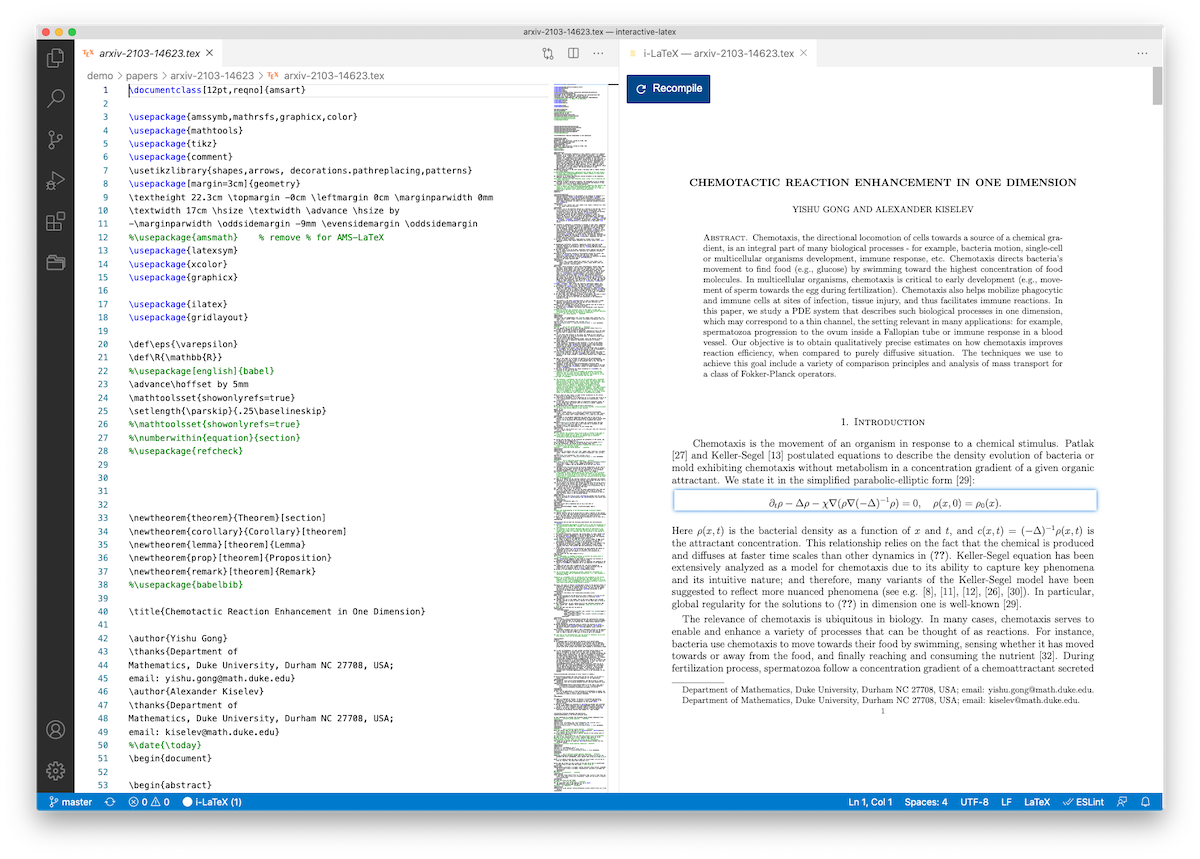
\includegraphics[width = \textwidth]{img/ilatex-editor-ui.png}
    \caption{A typical layout to edit a \LaTeX{} document opened with \iLaTeX{}: the code of the document is on the left, and the interactive PDF is on the right.}
    \label{fig:ilatex-ui}
\end{figure}
\section{Travaux connexes}
\label{sec:travaux-connexes}

Nous présentons les divers travaux ayant inspiré le concept de RII et le prototype \iLaTeX{} : les documents composés d'éléments interactifs ou programmables ; les langages, paradigmes et environnements de programmation non-textuels ; et les représentations intermédiaires utilisées dans d'autres domaines.


\subsection{Éditeurs de documents \LaTeX{}}

\LaTeX{} est un langage de description de document créé par Leslie Lamport en 1984~\cite{lamport1994latex} qui repose sur \TeX{}, un système de composition de document développé par Donald Knuth à la fin des années 1970~\cite{knuth1984texbook}.
Aujourd'hui, il demeure un choix courant pour la rédaction de publications académiques et techniques, et ce en dépit de la difficulté à l'utiliser --- y compris pour des utilisateurs experts, qui peuvent \og subir une perte de productivité lorsque \LaTeX{} est utilisé, par rapport à d'autres systèmes de préparation de{} documents \fg~\cite{knauff2014efficiency}.
Étant donné que \LaTeX{} est un langage de commandes, la plupart des éditeurs de documents \LaTeX{} ressemblent plus à des éditeurs de code qu'à des éditeurs WYSIWYG --- incluant des fonctionnalités telles que la coloration syntaxique et l'auto-complétion.
Certains éditeurs \LaTeX{} essaient d'offrir une expérience se rapprochant de celle des éditeurs WYSIWYG ; mais à notre connaissance, soit ils ne fournissent qu'un formatage de base du code source (\eg{} AUC\TeX{}\footnote{\url{https://www.gnu. org/software/auctex/}}, le mode \emph{rich text} d'Overleaf\footnote{\url{https://www.overleaf.com}}), soit ils fournissent une interface entièrement WYSIWYG qui masque le code et ne prend en charge qu'un ensemble limité de fonctionnalités (\eg{} Compositor\footnote{\url{https://compositorapp.com/}}).
Les éditeurs LyX\footnote{\url{https://www.lyx.org/}} et TeXmacs\footnote{\url{https://www.texmacs.org}} proposent de représenter un document entier sous une forme graphique intermédiaire mettant en avant sa structure et son contenu plutôt que son rendu final --- un paradigme souvent appelé \emph{What You See Is What You Mean}.
Néanmoins, à notre connaissance, aucun éditeur de ce type ne permet de manipuler directement le code \LaTeX{} (au delà de l'import/export au format \LaTeX{} et de l'insertion de courts morceaux de code, \eg{} une formule mathématique écrite en \LaTeX{}).
Plusieurs solutions permettent de pré-visualiser le rendu de certains éléments isolés (\eg{} une formule mathématique, une figure), d'animer la génération du document (\eg{} Gliimpse~\cite{dragicevic2011gliimpse}), ou encore d'associer à chaque élément du PDF généré une position dans le code, et inversement (\eg{} SyncTeX~\cite{laurens2008direct}) ; mais aucune d'entre elles ne permet de modifier le code plus facilement.

\iLaTeX{} se distingue des éditeurs de documents \LaTeX{} existants en offrant un accès immédiat et complet au code \LaTeX{} et au PDF généré (à la façon des éditeurs de code comme TeXstudio) tout en permettant de visualiser et de manipuler le code de certains éléments à travers des représentations plus adaptées plus ou moins similaires à celles imposées par des éditeurs comme LyX et Compositor.



\subsection{Documents interactifs}

Dans son essai de 2011, \emph{Explorable Explanations}\footnote{\url{http://worrydream.com/ExplorableExplanations/}}, Bret Victor plaide en faveur de documents plus interactifs, dans lesquels les utilisateurs pourraient dynamiquement modifier des valeurs et observer comment d'autres informations évoluent.
Ce principe est repris par les multivers de Dragicevic~\etal{}~\cite{dragicevic2019increasing}, qui démontrent l'intérêt de permettre aux lecteurs d'explorer différentes façons d'analyser et de visualiser des données expérimentales.
Afin de rendre la conception de documents interactifs plus accessible aux non-programmeurs, Conlen~\etal{} présentent Idyll~\cite{conlen2018idyll}, un langage de balises conçu pour les journalistes.
Afin d'outrepasser le manque d'interactivité lié aux limites de certains formats de fichiers, Chameleon~\cite{masson2020chameleon} propose d'identifier certains contenus sur l'écran à l'aide de techniques de vision par ordinateur afin d'y surimprimer des versions animées ou interactives du même contenu.

En permettant de modifier le code source des documents en interagissant avec le PDF, \iLaTeX{} exploite la notion de document interactif.
Cependant, contrairement aux travaux présentés ci-dessus, il ne s'agit pas de produire un document PDF interactif pour les \emph{lecteurs}, mais de rendre son édition plus interactive pour les \emph{auteurs}.



\subsection{Programmation de documents}

L'idée de mélanger rédaction de documents et programmation est apparue avec le développement de nouveaux langages de description de document dans les années 1970.
Elle s'est poursuivie par la promotion de concepts tels que le \emph{literate programming}~\cite{knuth1984literate} de Knuth et la conception de langages et de paradigmes de programmation centrés sur l'humain (tels que Smalltalk~\cite{goldberg1983smalltalk80}) dans les années 1980.
Cette idée a depuis été remise au goût du jour par la popularité croissante des \emph{computational notebooks} comme Jupyter\footnote{\url{https://jupyter.org/}}, largement adoptés par des communautés de sciences des données.
Les \emph{notebooks} permettent de faire cohabiter des cellules dont le contenu est rédigé par les auteurs (texte, code) avec des cellules dont le contenu est généré par l'exécution d'un programme.
Bien que ces dernières soient traditionnellement statiques, Kery~\etal{}~\cite{kery2020future} présentent plusieurs pistes pour rendre celles-ci plus interactives --- par exemple pour les tableaux de données ({Figure~\ref{fig:interactive-dataframe-exemple}}).
Wrex~\cite{drosos2020wrex} permet de synthétiser le code permettant d'insérer et de remplir une nouvelle colonne à partir d'un ou plusieurs exemples fournis interactivement par les utilisateurs via la représentation d'un tableau de données.

\iLaTeX{} inclut un éditeur de code et permet donc naturellement d'utiliser toutes les fonctionnalités de programmation de document offertes par \LaTeX{}.
Les représentations intermédiaires qu'il inclut constituent un moyen supplémentaire de
visualiser et de manipuler le code, au même titre que celles développées pour les \emph{notebooks} sus-mentionnés.

\begin{figure}
    \centering
    \iincludegraphics[width=0.4\textwidth]{interactive-dataframe.png}
    \caption{Déplacer une colonne du tableau génère le code qui implémente la modification (adapté de Kery \etal~\cite{kery2020future}).}
    \Description{L'image contient deux étapes d'une même interaction : cliquer et déplacer la colonne d'un tableau (représentant un dataframe dans un notebook) pour l'insérer entre deux autres colonnes. La seconde étape montre le résultat une fois la colonne déplacée, et le tableau est désormais précédé d'une cellule contenant un commentaire "generated code" et quatre lignes de code Python qui extraient la colonne déplacée, puis la réinsèrent à sa nouvelle position.}
    \label{fig:interactive-dataframe-exemple}
\end{figure}



\subsection{Programmation non-textuelle}

Depuis les années 1980, des langages de programmation visuels particulièrement adaptés au traitement de signaux multimédia tels que Max\footnote{\url{https://cycling74.com/products/max}} et Pure Data\footnote{\url{https://puredata.info/}} ont été développés.
La syntaxe graphique simple et la manipulation directe des blocs qui composent les programmes rendent ces langages particulièrement accessibles à des utilisateurs sans formation en programmation.
Cela pourrait expliquer pourquoi ce type de langage continue d'être utilisé aujourd'hui.
Il a par exemple été choisi pour concevoir Dynamic Brushes~\cite{jacobs2018extending}, un système de programmation du comportement d'un pinceau numérique destiné à des illustrateurs.
D'autres langages visuels ont également été largement adoptés à des fins éducatives (\eg{} Scratch~\cite{resnick2009scratch}).
Néanmoins, certains chercheurs affirment qu'ils pourraient également être utiles pour des professionnels~\cite{bau2017learnable}.
Dans cette optique, Droplet\footnote{\url{http://droplet-editor.github.io/}} et les \emph{frame-based editors}~\cite{brown2016framebased} illustrent deux façons de 
faire fusionner la richesse des langages textuels avec la manipulation directe des langages à blocs.

La programmation non-textuelle peut également prendre la forme de nouveaux genres d'éditeurs de code.
Plusieurs travaux proposent d'aider les programmeurs à visualiser l'état courant du programme en augmentant des éditeurs de code traditionnels avec des données brutes~\cite{lerner2020projection} ou visualisées~\cite{hoffswell2018augmenting}.
Python Tutor~\cite{guo2013online} affiche par exemple les structures de données utilisées sous une forme schématique à des fins éducatives.
D'autres travaux portent plutôt sur de nouvelles façons d'interagir avec le code.
Sketch-n-Sketch~\cite{hempel2019sketchnsketch} est un éditeur expérimental permettant de programmer une image vectorielle en utilisant un langage fonctionnel et de modifier son code en interagissant directement avec le SVG généré.
Il illustre l'idée du \emph{output-directed programming} de Chugh~\cite{chugh2016programmatic}, qui consiste à éditer le code source d'un programme en manipulant directement sa sortie graphique.

Les représentations intermédiaires de \iLaTeX{} sont inspirées de ces différentes façons de penser le code autrement que comme du texte brut --- et plus particulièrement de l'approche de Sketch-n-Sketch.
Ces représentations permettent de s'affranchir de la compilation du document pour visualiser le moindre changement tout en permettant de donner forme à des abstractions invisibles dans le code et effacées dans le document généré.



\subsection{Représentations intermédiaires}

La représentation la plus appropriée du code d'un programme ou d'une description de document peut se situer entre le code brut et la sortie du programme : on parle alors de représentation \emph{intermédiaire}.
Si celle-ci permet de modifier le code qu'elle représente, elle est de surcroît \emph{interactive} ({Figure \ref{fig:intermediate-representations-examples}}).
Barista~\cite{ko2006barista}, Envision~\cite{asenov2014envision} et JetBrains MPS\footnote{\url{https://www.jetbrains.com/mps/}} sont différents éditeurs de code capables d'afficher certains éléments de langages textuels sous une forme structurée (\eg{}~organiser le code sous forme d'un tableau) ou graphique (\eg{} dessiner les symboles d'une expression mathématique).
Graphite~\cite{omar2012active} permet de générer le code d'une couleur à partir d'une palette interactive, tandis que Clint~\cite{zinenko2014clint} permet de modifier le code de boucles imbriquées afin d'améliorer les performances d'un programme à travers la manipulation de diagramme interactifs.

\iLaTeX{} a pour but de fournir des représentations intermédiaires de morceaux de code \LaTeX{} qui gagnent à pouvoir être visualisés et manipulés autrement que sous forme textuelle, de la même manière que des systèmes tels que Barista et Clint le font pour des langages de programmation et des paradigmes plus traditionnels.
En outre, \iLaTeX{} permet d'afficher ces visualisations à proximité des éléments correspondants du PDF généré, renforçant ainsi les liens entre les deux ; tandis que les exemples donnés ci-dessus les affichent généralement uniquement à proximité du code concerné.

\begin{figure*}[ht]
    \center
    \subfigure[Éditeur d'animation de Mozilla Firefox]{%
        \centering\iincludegraphics[width=0.4\textwidth]{firefox-anim-editor.png}
        \label{subfig:firefox-anim-editor}
    }
    \subfigure[Éditeur de boucles imbriquées de Clint (d'après Zinenko \etal~\cite{zinenko2015manipulating})]{%
        \centering\iincludegraphics[width=0.4\textwidth]{clint.png}
        \label{subfig:clint}
    }
    \caption{Exemples de représentations intermédiaires interactives. \psubref{subfig:firefox-anim-editor} La manipulation des poignées pour modifier la courbe met à jour les paramètres numériques de la propriété CSS (affichée en dessous). \psubref{subfig:clint} L'inclinaison du polygone transforme le code C++ (affiché au dessus) pour refléter la façon dont les opérations doivent être parallélisées selon le nouveau diagramme.}
    \Description{Deux interfaces contenant des représentations intermédiaires. L'interface (a) contient une dizaine de miniatures de courbes représentant des possibilités de progression d'animation, ainsi que la courbe représentant la progression courante avec deux poignées permettant de la déformer. L'interface (b) contient deux graphiques 2D (avant et après transformation). Chaque graphique contient un ensemble de points (itérations) relié par des flèches représentant leurs dépendances (contraintes sur l'ordre des calculs). Le passage d'un graphique à l'autre déforme le polygone qui contient tous les points.}
    \label{fig:intermediate-representations-examples}
\end{figure*}
\section{Interviews d'utilisateurs de \LaTeX{}}
\label{sec:interviews}

Afin de mieux comprendre de quelles façons les RII pourraient améliorer l'édition de langages de description de document, nous avons interviewé 11 utilisateurs de \LaTeX{} et réalisé une analyse thématique des difficultés que ceux-ci rencontrent.
Dans cette section, nous présentons la méthodologie utilisée et les résultats obtenus.
À notre connaissance, aucune étude similaire n'a déjà été publiée.


\subsection{Méthodologie}

\subsubsection{Participants}
Nous avons interviewé 11 participants (5~femmes et 6~hommes, âgés de~21 à~40 ans).
La plupart sont des étudiants de Master (8/11) ou des personnes issues du milieu universitaire, spécialisés dans des domaines très divers.
Les participants ont été recrutés via un mailing interne au laboratoire et un message sur un groupe Facebook d'une grande école.
Ils n'ont reçu aucune compensation pour leur participation.
Chacun d'entre eux avait utilisé \LaTeX{} au cours des semaines ou des mois précédant leur interview.
Les participants ont l'habitude d'utiliser Overleaf (5/11) ou Texmaker (5/11) pour rédiger des documents \LaTeX{}, mais plusieurs d'entre eux ont également utilisé ou essayé au moins un éditeur alternatif parmi TeXstudio, TeXworks, Kyle et Gedit --- sur Windows, MacOS ou Linux.
En outre, la majorité d'entre eux utilise également des logiciels de traitement de texte.
Leur expertise avec \LaTeX{} est très variable\footnote{Les niveaux d'expertise sont définis de la façon suivante : les \emph{débutants} ne se sentent pas à l'aise avec \LaTeX{} et ont besoin d'aide pour utiliser la plupart des fonctionnalités ; les utilisateurs \emph{intermédiaires} se sentent à l'aise pour écrire des documents simples avec quelques structures et mettre le texte en forme ; et les utilisateurs \emph{avancés} se sentent à l'aise pour inclure du contenu varié et créer leurs propres commandes. Chaque participant a été invité à auto-évaluer son niveau d'expertise, que nous avons ensuite adapté en fonction des fonctionnalités avec lesquelles il se sentait à l'aise ou non.}, mais la plupart des participants (8/11) sont des utilisateurs intermédiaires.
Des informations supplémentaires sur chaque participant peuvent être trouvés dans la {Table~\ref{tab:participants}}.

\begin{table*}[h]
    \centering
    \makebox[\textwidth]{\begin{itabular}{lllll}
        \toprule
        Participant & Profession & Domaine & Expertise & Principal document présenté \\
        \midrule
        P1 & Étudiante en Master & Biologie & Intermédiaire & Rapport de stage \\
        P2 & Doctorante & Visualisation de données & Intermédiaire & Thèse de doctorat \\
        P3 & Étudiant en Master & Écologie & Intermédiaire & Devoir à rendre \\
        P4 & Étudiante en Master & Géologie & Intermédiaire & Projet de hackathon \\
        P5 & Enseignant-chercheur & Informatique & Avancé & Article de mathématiques \\
        P6 & Étudiant en Master & Systèmes complexes & Intermédiaire & Sujet de thèse \\
        P7 & Étudiante en Master & Géochimie & Intermédiaire & Rapport de stage \\
        P8 & Étudiante en Master & Archéologie & Débutant & Rapport de stage \\
        P9 & Étudiant en Master & Informatique & Intermédiaire & Article d'informatique \\
        P10 & Professeur de lycée & Philosophie & Intermédiaire & Liste d'examens de philo. \\
        P11 & Étudiant en Master & Informatique & Avancé & Notes de cours de math. \\
        \bottomrule
    \end{itabular}}
    \caption{Détails sur les participants interviewés.}
    \label{tab:participants}
\end{table*}


\subsubsection{Procédure}
Toutes les interviews étaient semi-structurées, menées en français, et d'une durée moyenne d'une heure environ (entre 29 et 99 minutes).
La durée des interviews et le choix des questions ont été ajustés à l'aide de trois interviews pilotes de collègues doctorants et post-doctorants.

Nous avons commencé chaque interview en demandant à chaque participant de nous montrer le dernier document \LaTeX{} sur lequel il avait travaillé via un partage d'écran (comprenant à la fois le code \LaTeX{} et le PDF généré).
Nous leur avons tout d'abord posé plusieurs questions relatives au document présenté (\eg{} type de document, éditeur utilisé, etc).
Nous leur avons ensuite demandé de nous décrire les différents problèmes auxquels ils avaient fait face (qu'ils les aient résolus ou non) en se référant le plus possible au code du document (dans le double but de les aider à s'en souvenir et de rendre leurs explications plus claires pour nous).
Les interviews étant semi-structurées, nous avons utilisé une liste de questions prédéfinies pour guider les participants, mais ceux-ci étaient invités à parler librement de chaque problème rencontré.
Les participants étaient également invités à nous parler de problèmes rencontrés sur d'autres documents si cela leur semblait pertinent.
Nous avons conclu chaque interview avec quelques questions plus générales sur l'expérience de chaque participant avec \LaTeX{}.

\subsubsection{Données récoltées}
Toutes les interviews ont été enregistrées (audio et écran partagé) et retranscrites manuellement, incluant de courtes descriptions du contenu affiché à l'écran ou des interactions des participants lorsque cela était pertinent.
Nous avons également pris des notes manuscrites synthétisant les problèmes principaux et les solutions utilisées.

\subsubsection{Analyse des données}
\label{sssec:collecte-analyse-donnees}
Nous avons réalisé une analyse thématique~\cite{braun2019reflecting} à partir des données récoltées.
Le premier auteur a tout d'abord généré plus de 650 codes à partir des huit premières transcriptions, qu'il a ensuite classés dans près de 80 sous-thèmes.
Nous nous sommes alors servis de ces sous-thèmes afin de générer trois jeux de thèmes :
un premier jeu regroupant les sous-thèmes similaires (\ie{} des \emph{domain summaries}, dans le vocabulaire de Braun et Clarke) ;
un second jeu regroupant les problèmes similaires (indépendamment du contexte dans lequel ils sont apparus) ;
et un troisième jeu issu d'un mélange des deux premiers.

Ce dernier jeu a été élaboré à l'aide de discussions avec plusieurs chercheurs de l'équipe dans le but d'identifier les groupes de sous-thèmes les plus pertinents dans les deux premiers thèmes.
Nous avons également réécouté les trois interviews non-transcrites afin de nous assurer de leur inscription dans les cinq thèmes finaux, et nous en avons extrait plusieurs citations afin de renforcer et de contraster ce qui avait déjà été mis en évidence par les huit premières interviews.
Nous présentons le contenu des cinq thèmes finaux ci-dessous.




\subsection{Résultats}

\subsubsection{T1 --- Le code source doit être accessible et modifiable}

\paragraph{Les interfaces WYSIWYG sont limitées}
En dépit des difficultés que cela induit, la plupart des participants semblent à l'aise avec le paradigme consistant à décrire leur document dans un langage particulier ; et peu ont évoqué le désir d'un éditeur WYSIWYG pour \LaTeX{}.
P2 craint par exemple que déplacer des morceaux de texte dans Microsoft Word \citeparticipant{[fasse] du code dégueu\textasteriskcentered\textasteriskcentered\textasteriskcentered\textasteriskcentered\textasteriskcentered{} derrière}, tandis que P4 a expliqué se sentir \citeparticipant{impuissante} lorsqu'elle ne peut pas obtenir ce qu'elle veut dans un éditeur WYSIWYG.
À l'exception de P7, aucun de ceux qui connaissaient le mode \emph{rich text} d'Overleaf ne l'utilisent.
Plusieurs participants lui reprochent de manquer de fonctionnalités en cachant le code, impliquant ainsi \citeparticipant[P8]{plus de manipulation, plus de mouvement sur l'écran} afin de régulièrement passer d'un mode à l'autre.
P7 a d'ailleurs reconnu qu'elle l'avait uniquement utilisé pour prendre des notes pendant un cours d'histoire : \citeparticipant[P7]{il fallait juste taper ; j'avais pas de maths à faire ; j'avais pas de photo à rajouter}.

\paragraph{Le document doit pouvoir être programmé}
Plusieurs participants parmi les plus experts ont expliqué qu'ils aimaient pouvoir créer des commandes personnalisées pour générer ou réutiliser du contenu (\eg{} développer des abréviations, réutiliser un dessin paramétré).
Au fil des années, P11 s'est par exemple constitué un long préambule contenant plusieurs dizaines de commandes personnalisées pour générer des expressions mathématiques (telles que les noms de théorèmes et des constructions courantes), qu'il continue d'utiliser.
P10 explique avoir choisi \LaTeX{} pour créer une archive unique de centaines d'examens de philosophie de lycée, car il souhaitait pouvoir générer plusieurs index (par auteur, par thème, par type de question philosophique, etc) qui seraient automatiquement mis à jour s'il ajoutait de nouveaux examens par la suite.
Selon lui, un tel niveau d'automation est impossible à atteindre avec un système de préparation de document de type WYSIWYG : \citeparticipant[P10]{sous LibreOffice, on ne peut avoir un index alphabétique que pour une seule catégorie}.
La nature textuelle de \LaTeX{} permet également de générer des documents de toute pièce facilement.
P5 a ainsi écrit un programme Python pour générer un code \LaTeX{} représentant plusieurs centaines de badges similaires pour un concours de Go : \citeparticipant[P5]{Si vous me demandez de vous faire deux cent badges en Word, vous vous démer\textasteriskcentered\textasteriskcentered\textasteriskcentered{}~; je le fais pas}.

\paragraph{Les commentaires ont de multiples utilités}
Seule une fraction des participants a déclaré utiliser des commentaires dans le code ; mais ceux qui s'en servent expliquent que leur utilité est multiple.
Les raisons de s'en servir incluent
(1) se rappeler de l'utilité d'un paquet ou d'une commande ;
(2) discuter avec d'autres co-auteurs ;
(3) conserver des morceaux de code inutilisés qui pourraient servir plus tard ;
(4) commenter le code afin de trouver la source d'une erreur ;
(5) réutiliser des extraits d'un ancien morceau de code pour en écrire une nouvelle version ;
ou encore (6) planifier le contenu à écrire dans chaque partie du document.

\paragraph{L'accès au code facilite la réutilisation}
P5 a expliqué que le fait d'avoir accès au code permettait de copier-coller immédiatement des solutions trouvées sur internet, sans avoir à reproduire les étapes énumérées dans un tutoriel destiné aux éditeurs WYSIWYG.
Cet accès lui permet également de réutiliser le code \LaTeX{} de ses articles scientifiques afin de créer des présentations pour des colloques.



\subsubsection{T2 --- Apprendre \LaTeX{} est compliqué et chronophage}

\paragraph{\LaTeX{} est difficile à apprendre}
La plupart des participants ont expliqué qu'ils attendaient généralement de rencontrer des problèmes pour se renseigner sur \LaTeX{} et ses fonctionnalités.
Plusieurs ont souligné que cela arrivait souvent dans des moments de hâte, peu avant un rendu --- ne leur laissant donc pas la possibilité de prendre le temps de comprendre le code qu'ils devaient utiliser (après l'avoir copié-collé) : \citeparticipant[P2]{Pour l'instant je suis plus dans l'optique que ça doit marcher}.
Le nom des commandes, l'ordre de leurs paramètres, et les valeurs autorisées pour ces derniers semblent souvent être oubliés ou ignorés par les participants --- y compris lorsqu'ils ont déjà l'habitude de s'en servir : \citeparticipant[P3]{Je saurais qu'il faut une minipage, mais je serais quand même obligé d'aller chercher quelque part comment l'écrire}.

\paragraph{Ne pas comprendre \LaTeX{} est coûteux}
Certains participants ont reconnu que leur incompréhension de \LaTeX{} était parfois coûteuse : \citeparticipant[P7]{[Personnaliser] la biblio, c'est le truc qui était le plus long, parce que j'ai pas trouvé de solution toute faite quoi. Il a fallu que j'invente un petit peu \elips{}}.
P2 et P4 ont exprimé des regrets de n'avoir jamais eu de cours sur \LaTeX{} avant de devoir l'utiliser : \citeparticipant[P2]{J'aurais voulu prendre une journée [pour apprendre \LaTeX{}] ; il y a des formations qui présentent les bases}.
P6 a au contraire expliqué qu'il ne voudrait pas faire un tel effort : \citeparticipant[P6]{Tu trouves un document qui marche, tu copies-colle, et tu changes par itération \elips{} je vais pas apprendre la structure du code.}

\paragraph{Les recherches portent sur des problèmes spécifiques}
Les participants ont indiqué qu'ils cherchaient souvent des solutions à des problèmes spécifiques : produire un symbole particulier, comprendre une erreur, trouver la documentation d'un paquet, etc.
Lorsqu'il a eu besoin de poursuivre la numérotation d'une liste, P3 a par exemple rapidement trouvé la solution sur internet : \citeparticipant[P3]{j'ai trouvé que c'était après le \texttt{\symbol{92}begin\string{enumerate\string}} qu'il fallait mettre le start, égal, ce qu'on veut}.
Néanmoins, trouver une réponse ne semble pas toujours être évident pour tous les participants.
Afin de trouver une solution pour insérer du grec ancien dans son document \LaTeX{}, P8 a par exemple expliqué avoir \citeparticipant[P8]{plutôt cherché sur des trucs de linguistique et d'historien} --- où elle n'a pas pu trouver de réponse.



\subsubsection{T3 --- Les éditeurs textuels sont inadaptés au contenu structuré}

\paragraph{Les éditeurs de code ignorent les structures}
De nombreux participants se sont plaints de la difficulté de décrire des éléments structurés tels que des tableaux, des sous-figures, ou même des formules chimiques.
La création de tableaux a souvent été décrite comme \citeparticipant[P1]{vachement chi\textasteriskcentered\textasteriskcentered\textasteriskcentered{}}, et la difficulté de leur édition leur a été reprochée : \citeparticipant[P3]{ça m'est arrivé de devoir déplacer des colonnes \elips{} ça se fait, mais c'est juste que ça prend du temps}.
Selon P7, à cause de la syntaxe des tableaux, \citeparticipant{oublier une colonne c'est un enfer} car \citeparticipant[P7]{il faut que je rajoute des trucs et qu'à chaque ligne je compte, je me mette au bon endroit}.
Ces observations s'appliquent également à d'autre types de contenu structuré, en particulier lorsque les participants ne sont pas familiers avec un paquet offrant une solution clé en main : \citeparticipant[P4]{L'autre truc qui est vraiment difficile aussi, c'est de mettre les images côte à côte}.

\paragraph{Le recours aux outils externes}
En raison des difficultés à créer et modifier du contenu structuré depuis leurs éditeurs \LaTeX{}, plusieurs participants se tournent vers des outils externes.
P2 et P4 ont par exemple toutes deux commencé par utiliser des sous-figures constituées d'images séparées dans \LaTeX{} avant de finalement les fusionner en utilisant Inkscape ou Adobe Illustrator car \citeparticipant[P2]{comme ça je maîtrisais la mise en page}.
Afin de créer des tableaux à partir de classeurs Excel, P7 les a exportés au format CSV afin de générer le code \LaTeX{} correspondant en utilisant le convertisseur en ligne \url{tablesgenerator.com}.
Elle a cependant expliqué avoir dû répéter le processus à chaque fois qu'elle souhaitait modifier les tableaux, dont le code généré était trop difficile à interpréter sous forme de texte brut.
D'autres participants ont par ailleurs indiqué qu'ils utilisaient ce même site web pour créer des tableaux \LaTeX{} à partir de zéro.
P7 s'est également plainte de ne pas pouvoir exporter les structures créées dans des logiciels spécialisés tels que Microsoft Excel (pour les tableaux) ou ChemDraw (pour les molécules) sous forme de code \LaTeX{} --- soulignant là encore à quel point les éditeurs de code sont inadaptés pour décrire et manipuler certaines structures :
\citeparticipant{un truc qui serait utile c'est de dessiner ma molécule de A à Z et que le code s'affiche à côté quoi}, car \citeparticipant[P7]{le truc le plus difficile que j'ai jamais utilisé sous \LaTeX{} c'est le package pour faire les molécules chimiques}.



\subsubsection{T4 --- Les abstractions sont difficiles à visualiser et à formaliser}

\paragraph{Les dimensions}
De nombreuses commandes \LaTeX{} requièrent de spécifier des dimensions, comme par exemple la taille d'une image ou les marges de certains éléments.
Or, selon plusieurs participants, les dimensions de \LaTeX{} souffrent de deux problèmes :
il est difficile de quantifier une longueur que l'on imagine, et il est difficile d'imaginer une longueur quantifiée.
\citeparticipant[P8]{Je ne sais pas forcément quelle taille précise je veux que l'image ait, mais [je sais] que je veux qu'elle ait cette taille-là dans ma tête}.
Comme de nombreux autres participants, P1 s'est aussi plainte de devoir essayer plusieurs dimensions jusqu'à trouver celle qui convient --- une stratégie parfois coûteuse : \citeparticipant[P1]{quand tu veux que [tes figures] soient un peu plus grosses, un peu plus petites, tu compiles quinze mille fois et c'est chi\textasteriskcentered\textasteriskcentered\textasteriskcentered{}~\elips{} surtout quand tu as beaucoup de figures, et que du coup il met beaucoup de temps à compiler}.
La plupart des participants semblent donc favorables à une forme d'interaction plus directe avec les dimensions.
Afin d'outrepasser ces difficultés, certains participants ont fait le choix de détourner des commandes avec lesquelles ils se sentent plus familiers.
P3 a ainsi inséré du texte de couleur blanche dans son document afin de sauter \citeparticipant{artificiellement} plusieurs lignes successives : \citeparticipant[P3]{je pense qu'il y avait une façon plus simple de le faire, mais comme j'étais assez pressé c'est comme ça}.

\paragraph{Les positions}
Au contraire des dimensions, \LaTeX{} se charge traditionnellement de calculer les positions des éléments à la place de l'utilisateur.
Cependant, selon certains participants, ce manque de contrôle n'est pas toujours souhaitable.
P1 a par exemple expliqué que sa façon de positionner les figures n'était \citeparticipant[P1]{pas très rationnelle}, et P2 s'est plainte de la difficulté de placer une image suffisamment près d'un paragraphe y faisant référence lorsque \LaTeX{} en décidait autrement.
Ces difficultés sont probablement renforcées par le fait que plusieurs participants ne sont pas conscients du sens des paramètres de positionnement qu'ils utilisent (\eg{} avec l'environnement \texttt{figure}) --- souvent copiés avec le reste d'un morceau de code.
Par conséquent, P4 --- qui a pourtant lu \citeparticipant{comment le compilateur faisait pour placer les images} afin de gagner en contrôle sur leur positionnement --- a ainsi admis avoir dû revoir ses attentes concernant les positions des figures à la baisse.
Ces difficultés concernent également les positions plus locales.
Bien qu'il se sente à l'aise avec les commandes de dessin du paquet TikZ, P5 a expliqué qu'il aimerait bien pouvoir déplacer certains éléments de ses dessins au lieu \citeparticipant{d'essayer de deviner} les bonnes coordonnées ou de faire \citeparticipant{vaguement de la trigo} pour les calculer.



\subsubsection{T5 --- La dualité entre le code et le PDF est coûteuse}

\paragraph{Identifier le code d'un élément du PDF est difficile}
Certains participants se sont plaints de la difficulté de faire le lien entre un élément du PDF et le code l'ayant généré.
P5 et P9 ont tous deux du mal à (1) localiser le code d'une formule mathématique affichée dans le PDF et (2) trouver le symbole qu'ils veulent corriger à l'intérieur du code de celle-ci.
Afin de résoudre le premier problème, ils recherchent souvent un extrait du texte voisin de la formule dans leurs éditeurs de code, bien que P5 ait admis que cette technique échoue régulièrement.
Cette approche n'est pas sans lien avec l'absence de support de SyncTeX dans l'éditeur \LaTeX{} que P5 utilise.
Il a d'ailleurs expliqué qu'il aimerait en changer pour cette raison --- soulignant l'importance de ce genre d'outil.
En revanche, ni P5 ni P9 n'ont trouvé de solution au second problème : pour eux, modifier une formule mathématique implique systématiquement \citeparticipant[P9]{de relire le code \LaTeX{} sans relire le PDF}.

\paragraph{Compiler est un processus lent}
De nombreux participants se sont plaints du temps requis pour compiler leurs documents \LaTeX{}.
Essayer plusieurs alternatives (\eg{} différentes tailles pour une image) est ainsi coûteux, et les erreurs font perdre du temps : \citeparticipant[P5]{si on se trompe ça nous coûte quand même une minute}.
Certains participants ont élaboré des stratégies en conséquence.
Afin de compiler moins souvent, P1 a expliqué qu'elle distinguait rédaction et mise en forme : \citeparticipant[P1]{quand je suis dans une phase de rédaction \elips{} je tape juste et j'écris \elips{} mais quand je fais la forme j'ouvre toujours [l'éditeur de code et le PDF] à côté, pour compiler régulièrement}.
P5 a également donné l'exemple de la mise en cache d'images crées avec TikZ : \citeparticipant[P5]{tant qu'il n'y a pas de modification faite sur l'image, [l'outil] réinjecte l'image à la place du code TikZ}.

\subsection{Recommandations pour le design}
Cette analyse thématique révèle la variété des problèmes auxquels les utilisateurs de \LaTeX{} font face et suggère plusieurs opportunités pour améliorer le design des éditeurs de documents \LaTeX{}. Nous résumons celles-ci dans les quatre recommandations suivantes.

\paragraph{Conserver l'accès au code}
Nous considérons qu'aucune interface graphique ne peut complètement dissimuler le code d'un document \LaTeX{} sans brider ses utilisateurs (\eg{} en ne supportant pas certaines fonctionnalités). 
Nous recommandons donc de permettre aux utilisateurs de \LaTeX{} de lire et de modifier librement et facilement le code de leurs documents.
De plus, certains utilisateurs veulent pouvoir réutiliser du code facilement ou automatiser sa génération.

\paragraph{Cibler les problèmes spécifiques et courants}
Même si la majorité des participants n'était pas fermée à l'idée d'apprendre à utiliser \LaTeX{}, aucun d'entre eux ne peut ou ne veut y consacrer beaucoup de temps.
Nous recommandons donc de ne pas restreindre les éditeurs \LaTeX{} à des fonctionnalités génériques plutôt destinées aux experts (\eg{} l'auto-complétion de commandes, qu'il faut donc connaître), mais également de prendre en compte les problèmes et les besoins plus spécifiques mais courants (\eg{} tableaux, sous-figures, références) et d'aider les utilisateurs moins expérimentés et intermittents à trouver ou concevoir des solutions à leurs problèmes.

\paragraph{Donner forme aux abstractions invisibles}
Étant donné la nature entièrement textuelle de \LaTeX{}, nous recommandons d'aider les utilisateurs à (1) visualiser les structures et les abstractions codées sous forme de texte lorsqu'elles s'y prêtent et (2) manipuler ces dernières à l'aide d'interactions adaptées tout en maintenant la synchronisation du texte source.
Ces visualisations doivent viser à réduire le nombre de cycles de compilation en facilitant la constitution de représentations mentales du document.

\paragraph{Renforcer les liens entre code source et document généré}
Face à la dualité entre code et rendu d'un même document, nous recommandons d'améliorer la visibilité et la spécificité des liens qui unissent ces deux substrats (\eg{} faciliter l'identification et la modification de la commande responsable d'un symbole mathématique particulier dans le PDF).

Les représentations intermédiaires interactives nous semblent pouvoir répondre à certains des problèmes soulevés par cette analyse thématique en respectant les recommandations que nous proposons ci-dessus.
Nous avons ainsi développé \iLaTeX, un prototype d'éditeur \LaTeX{} doté de RII, que nous présentons dans la section suivante.
\section{Prototype}
\label{sec:prototype}

\subsection{Description}
\iLaTeX{} est un prototype d'éditeur de documents \LaTeX{} doté de représentations intermédiaires interactives.
Son interface ressemble à celle de la plupart des éditeurs \LaTeX{} traditionnels (code source à gauche, PDF généré à droite), mais certains éléments du PDF sont interactifs, de telle sorte qu'en cliquer un affiche la représentation intermédiaire associée au morceau de code qui l'a généré ({Figure~\ref{fig:ilatex-interface}}).
Cette visualisation peut alors être utilisée par les auteurs du document pour (1) visualiser des structures et des abstractions invisibles (\eg{} la grille d'un tableau sans bordure visible) et (2) modifier le code source du document (\eg{} réordonner les colonnes d'un tableau en manipulant sa grille).
Selon la position de l'élément cliqué sur l'écran, sa représentation intermédiaire est affichée au-dessus ou en-dessous de celui-ci, de façon à le laisser le plus visible possible.
Le reste du document est assombri jusqu'à ce que la représentation soit fermée en cliquant sur la croix ou sur le document assombri --- déclenchant alors une recompilation du document \LaTeX{} afin de mettre le PDF à jour.
En outre, chaque visualisation affiche le nom et la position du morceau de code visualisé dans son en-tête. Ceux-ci peuvent être cliqués afin d'afficher le code correspondant dans l'éditeur de code.
Nous avons implémenté trois types de RII : deux pour des éléments \LaTeX{} courants (images et tableaux), et une pour un élément personnalisé (une grille de mise en page).
Elles sont décrites plus en détail ci-après et illustrées par la {Figure~\ref{fig:ilatex-visualisations}}.

\begin{figure*}[h]
  \centering
  \iincludegraphics[width = \textwidth]{ilatex-interface.png}
  \caption{Interface du prototype. (1)~Éditeur de code; (2)~Pré-visualisation du PDF généré; (3)~Tableau disposant d'une RII (cliquable); (4)~Visualisation du code du tableau (affichée par dessus le PDF). La {Figure~\ref{fig:ilatex-visualisations}} illustre les différentes visualisations.}
  \label{fig:ilatex-interface}
\end{figure*}

\subsubsection{Détail des visualisations}

\paragraph{Images}
Les images sont détectées par l'utilisation de la commande \texttt{includegraphics} (telle que fournie par le paquet \texttt{graphicx}\footnote{\url{https://ctan.org/pkg/graphicx?lang=en}}).
La représentation intermédiaire d'une image ({Figure~\ref{subfig:ilatex-visualisation-image}}) affiche l'image à la même taille que l'image affichée dans le PDF.
Elle peut être redimensionnée (à l'aide de la molette de la souris) et rognée (en redimensionnant le masque représenté par le rectangle avec une bordure sombre et une poignée).
Ces manipulations mettent automatiquement à jour les paramètres de la commande en modifiant les valeurs des clés \texttt{width}, \texttt{height}, \texttt{trim} et \texttt{clip} (ou en les supprimant si elles ne sont plus nécessaires).
Cette visualisation répond principalement à la difficulté de visualiser et de formaliser des dimensions (\reftheme{4}), mais elle facilite également la découverte de certains paramètres utiles (\reftheme{2}).

\paragraph{Tableaux}
Les tableaux sont détectés par l'utilisation de l'environnement \texttt{tabular}.
Leur représentation intermédiaire ({Figure~\ref{subfig:ilatex-visualisation-tableau}}) affiche le contenu brut de chaque \og{} cellule \fg de l'environnement, qui peut être édité en double-cliquant sur la cellule.
Le type de chaque colonne est affiché dans une ligne d'en-tête, et les colonnes et les lignes peuvent être réordonnées en cliquant longuement sur leurs en-têtes respectives et en les déplaçant.
Cette visualisation permet de mettre en exergue une structure abstraite pouvant être invisible dans le PDF (\reftheme{4}).
Elle rend également des transformations telles que la réorganisation de colonnes beaucoup plus faciles qu'elles ne le seraient dans un éditeur de code (\reftheme{3}).

\paragraph{Grilles de mise en page}
Les grilles de mise en page sont détectées par l'utilisation de l'environnement \texttt{gridlayout}, un environnement personnalisé que nous avons développé afin d'illustrer l'utilité de \iLaTeX{} pour ce type de structure.
Il permet d'utiliser une grille de mise en page (constituée de lignes et de cellules), qui permet de disposer localement du contenu de type varié (\eg{} texte, images, tableaux) suivant une grille invisible.
La représentation intermédiaire ({Figure~\ref{subfig:ilatex-visualisation-grille}}) rend la grille visible.
Les cellules peuvent être redimensionnées horizontalement en faisant glisser leur bordure droite, et les lignes peuvent être redimensionnées verticalement en faisant glisser leur bordure inférieure.
En outre, cliquer une cellule affiche et sélectionne son contenu dans l'éditeur de code.
Cette visualisation supporte l'édition de contenu structuré (\reftheme{3}) et la représentation concrète d'abstractions telles que des dimensions relatives (\reftheme{4}).
Elle illustre également le potentiel de développement de nouvelles fonctionnalités pour \LaTeX{} dont l'utilisation serait plus difficile ou désagréable sans RII.


\begin{figure*}[h]
  \begin{gridlayout}{\textwidth}{10cm}
    \begin{row}{0.264}
      \begin{cell}{0.5}
        \raggedleft
        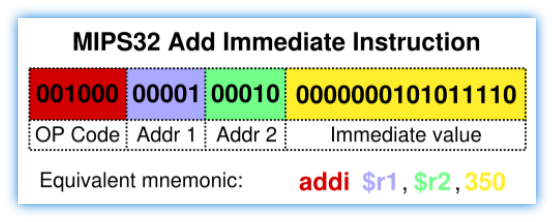
\includegraphics[height=\rowheight, width=\cellwidth, keepaspectratio]{image.png}
      \end{cell}
      \begin{cell}{0.5}
        \raggedright
        
\includegraphics[height=\rowheight, width=\cellwidth, keepaspectratio]{image-vis.png}
      \end{cell}
    \end{row}
    \begin{row}{0.268}
      \begin{cell}{0.5}
        \raggedleft
        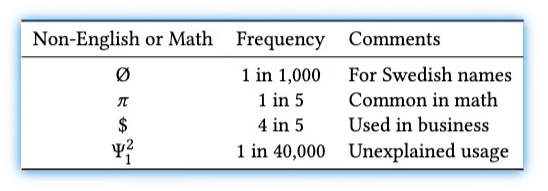
\includegraphics[height=\rowheight, width=\cellwidth, keepaspectratio]{table.png}
      \end{cell}
      \begin{cell}{0.5}
        \raggedright
        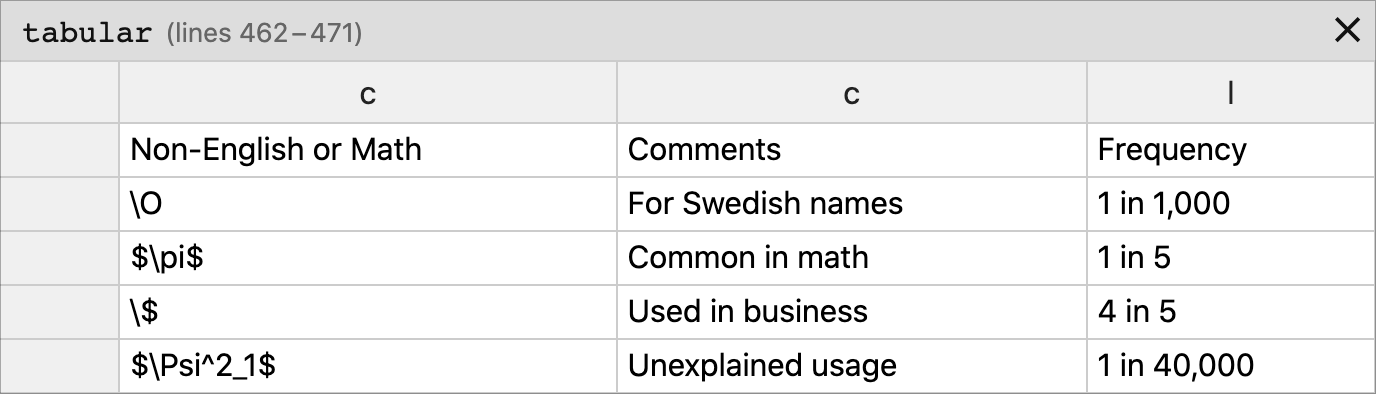
\includegraphics[height=\rowheight, width=\cellwidth, keepaspectratio]{table-vis.png}
      \end{cell}
    \end{row}
    \begin{row}{0.468}
      \begin{cell}{0.5}
        \raggedleft
        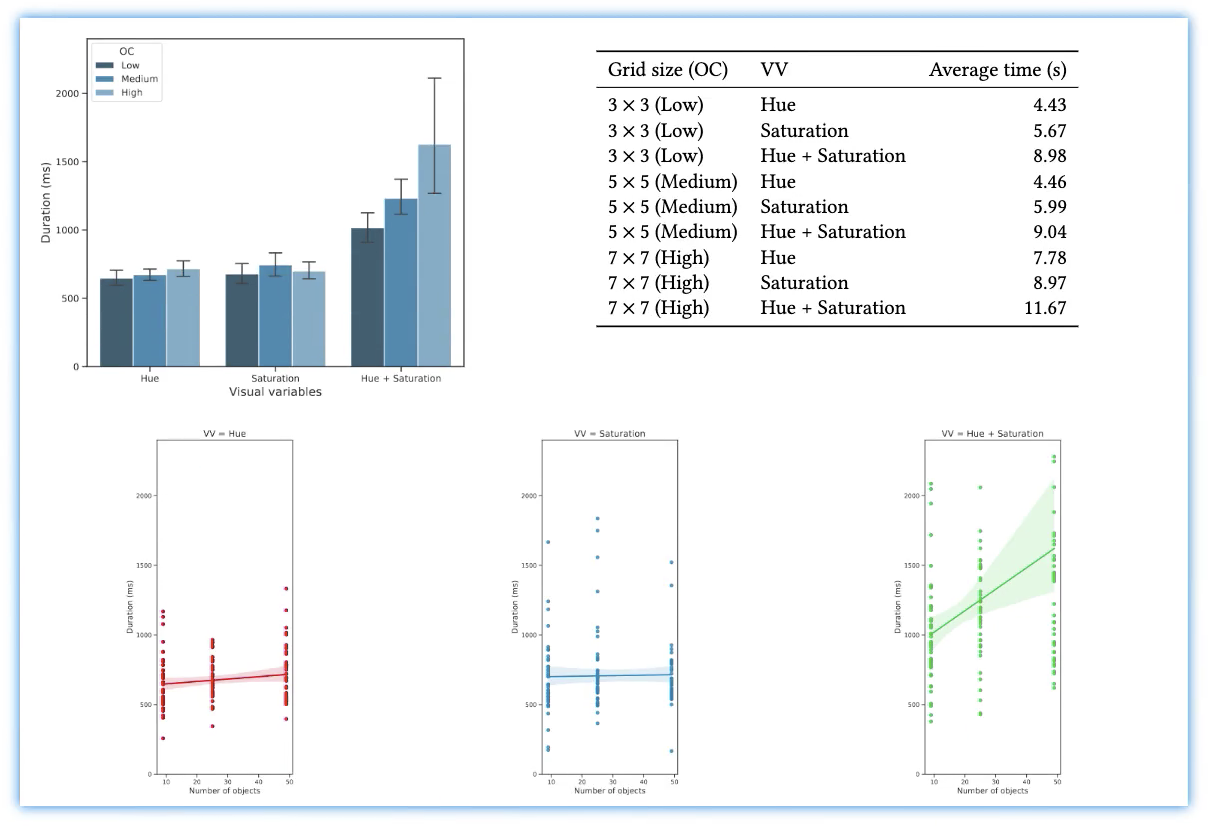
\includegraphics[height=\rowheight, width=\cellwidth, keepaspectratio]{grid-layout.png}
      \end{cell}
      \begin{cell}{0.5}
        \raggedright
        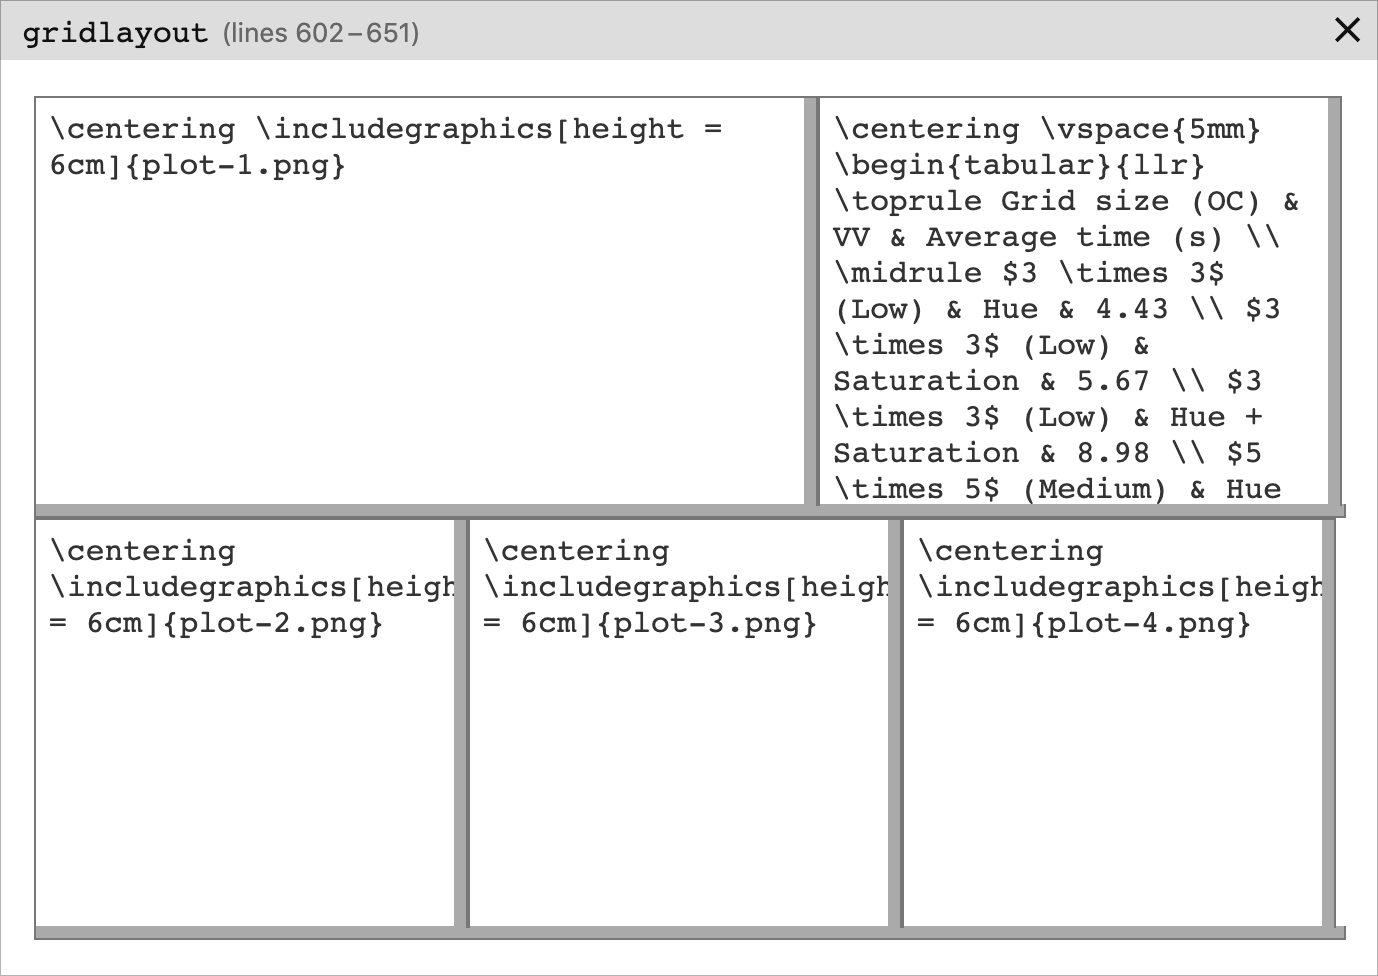
\includegraphics[height=\rowheight, width=\cellwidth, keepaspectratio]{grid-layout-vis.png}
      \end{cell}
    \end{row}
  \end{gridlayout}
  
  \caption{Exemples des visualisations disponibles dans \iLaTeX{}.
  Les éléments interactifs du PDF tels qu'ils apparaissent dans \iLaTeX{} sont affichés à gauche, et les visualisations du code les ayant générés sont affichées à droite (les images ne sont pas à l'échelle).
  Chaque visualisation ayant été modifiée, le code a déjà été mis à jour, et le document sera recompilé dès que la visualisation sera fermée. 
  \psubref{subfig:ilatex-visualisation-image} L'image a été rognée de façon à isoler le tableau central dans la visualisation --- d'où la région éclaircie en dehors du rectangle.
  \psubref{subfig:ilatex-visualisation-tableau} Les deux dernières colonnes ont été inversées dans la visualisation.
  \psubref{subfig:ilatex-visualisation-grille} La séparation entre les deux cellules de la première ligne a été déplacée vers la droite dans la visualisation.}
  \label{fig:ilatex-visualisations}
  \Description{Exemples d'une image, d'un tableau, d'une grille de mise en page et de leurs visualisations. La visualisation (a) contient une image dont une partie est sélectionnée dans un rectangle. La visualisation (b) contient le code des cellules du tableau sous forme de grille. La visualisation (c) contient le code de la grille sous forme d'une grille dont les dimensions sont proportionnées à celles de la grille issue du PDF.}
\end{figure*}



\subsection{Implémentation}
Le prototype est implémenté en tant qu'extension de l'éditeur Visual Studio Code\footnote{\url{https://code.visualstudio.com/}} (VSC), un éditeur de code open-source.
L'extension est écrite en TypeScript, HTML et CSS et organisée selon le patron de conception MVC.
Les particularités de son implémentation sont discutées ci-dessous.


\subsubsection{Extraction du code à visualiser}
Contrairement à la plupart des langages de programmation, \LaTeX{} n'est pas un langage hors-contexte, mais un langage récursivement énumérable (avec des caractéristiques peu communes telles que le concept de \emph{catcodes}, qui permet de modifier dynamiquement la signification de toute unité lexicale n'importe où dans le document).
En théorie, il est donc impossible d'écrire un analyseur syntaxique destiné à structurer le code que l'on souhaite visualiser en utilisant des outils traditionnellement dédiés à ce type de tâche.
Néanmoins, certaines conventions propres à \LaTeX{} demeurent très couramment utilisées (\eg{} la notion d'environnement).
En pratique, il est donc possible d'écrire un analyseur syntaxique qui accepte une proportion raisonnable de documents \LaTeX{} qui respectent lesdites conventions.

Pour les besoins du prototype, nous avons donc écrit un analyseur syntaxique de documents \LaTeX{} le plus générique possible dont le but est de fournir juste assez d'informations et de structure pour identifier les morceaux de code à visualiser, tels que certaines commandes spécifiques et leurs paramètres.
L'arbre de syntaxe abstraite ainsi généré est ensuite utilisé pour identifier les sous-arbres représentant des morceaux de code pertinents à visualiser (\eg{} un environnement nommé \texttt{tabular}).
Cette conception minimale a été choisie pour (1) maximiser le succès de l'analyse et (2) minimiser le temps d'exécution.
En contrepartie, chaque visualisation est responsable d'effectuer une analyse statique du code plus approfondie si nécessaire.


\subsubsection{Annotation du document PDF}
Le format de fichier PDF --- typiquement utilisé en sortie par les moteurs \LaTeX{} --- n'est pas conçu pour contenir des informations sur les régions du code \LaTeX{} à l'origine des différents éléments qui le composent.
Afin d'outrepasser cette limitation, nous avons choisi d'utiliser des annotations PDF contenant un identifiant unique et dont la boîte se superpose à celle de l'élément à associer à un morceau de code.
Celles-ci sont générées en englobant le morceau de code à visualiser dans une commande \texttt{ilatex} personnalisée\footnote{Bien que cela nécessite l'utilisation d'une commande spéciale pour le moment, il convient de noter que puisque tout peut être redéfini dans \LaTeX{}, les commandes et environnements existants pourraient être silencieusement modifiés afin que ceux-ci utilisent automatiquement la commande \texttt{ilatex}.}, comme dans \verb|\ilatex{\includegraphics{fig.pdf}}|.
Chaque utilisation de cette commande écrit également une nouvelle entrée dans un fichier regénéré à chaque compilation du document, qui contient des informations sur le morceau de code (\eg{} sa position dans le code) et sur la valeur courante de certaines macros (\eg{} \verb|\linewidth|).


\subsubsection{Affichage du PDF augmenté}
Une fois le document compilé en un PDF annoté, celui-ci est affiché à l'aide d'un moteur de rendu personnalisé (basé sur PDF.js\footnote{\url{https://github.com/mozilla/pdf.js/}}).
Celui-ci est responsable d'extraire toutes les annotations insérées par la commande \texttt{ilatex} et de les afficher sous forme de rectangles colorés autour des éléments disposant d'une visualisation.
Lorsque l'un d'eux est cliqué, \iLaTeX{} identifie le morceau de code auquel correspond l'annotation afin d'afficher la bonne visualisation.
Celui-ci est identifié en comparant l'identifiant attribué à l'annotation du PDF à ceux présents dans le fichier généré lors de la compilation du document.



\subsection{Évaluation préliminaire}
Étant donné la variabilité de l'expertise et des besoins de chaque utilisateur de \LaTeX{} (comme en attestent les différents profils des participants interviewés --- voir la {Table \ref{tab:participants}}), une étude quantitative de l'efficacité de \iLaTeX{} (\eg{} vitesse d'édition, nombre d'essais-et-erreurs) ne nous semble pas être très pertinente.
À l'inverse, une étude plus qualitative --- telle qu'une étude de terrain --- permettrait de mieux comprendre les contextes dans lesquels les RII sont préférées à l'édition du code et de découvrir des utilisations inattendues et des fonctionnalités manquantes.
Cependant, le contexte sanitaire en place depuis l'émergence de la pandémie de Covid-19 ne nous a pour l'instant pas permis d'organiser une telle évaluation.
En dépit de cela, une fois les interviews terminées, nous avons toutefois décidé de recueillir les avis des participants sur une vidéo d'une version précoce de \iLaTeX{} afin d'obtenir une première estimation de son potentiel.
Conscients du risque de biais dus à cette approche, nous avons fait particulièrement attention à ne pas parler du prototype ni de la notion de RII avant la fin de chaque interview.

\subsubsection{Méthodologie}
Nous avons présenté à chaque participant une vidéo d'un prototype de \iLaTeX{} d'une durée d'environ deux minutes.
Celle-ci présentait l'interface utilisateur du logiciel et l'utilisation de versions préliminaires des visualisations du code des images et des tableaux (semblables à celles présentées dans cette section).
La vidéo étant muette, nous expliquions chaque action en voix off à l'aide d'un script.
Une fois la vidéo terminée, nous avons demandé aux participants ce qu'ils avaient compris du système, s'ils aimeraient l'essayer, et s'il y avait d'autres types d'éléments du PDF ou de morceaux de code \LaTeX{} qu'ils souhaiteraient manipuler d'une façon similaire.
Ces évaluations ont été enregistrées dans les mêmes conditions que celles des interviews.

\subsubsection{Résultats}
La majorité des participants ont exprimé des réactions positives concernant la vidéo du prototype : \citeparticipant[P1]{Mais comment t'as codé ça ? C'est trop cool !} ; \citeparticipant[P7]{vend ton truc à Overleaf \elips{} qu'ils le rajoutent !}
Tous ont indiqué avoir compris le fonctionnement de \iLaTeX{}.
Plusieurs ont également fait la remarque que cela semblait facile à utiliser : \citeparticipant[P4]{c'est vachement intuitif, \elips{} ça fait référence à des compétences que les gens ont déjà} ; \citeparticipant[P8]{je pense que c'est plus user-friendly que juste modifier le code}.
Les utilisateurs les plus experts semblent eux aussi enthousiastes à l'idée d'utiliser le système.
P5 a d'ailleurs insisté sur le fait que \iLaTeX{} ne cherche pas à supprimer l'accès au code (\citeparticipant{si ce n'était pas comme ça je ne me verrais pas interagir avec}), et P11 a reconnu que \iLaTeX{} pourrait \citeparticipant[P11]{m'encourager à utiliser plus d'illustrations et de tableaux}.
En outre, P4 a souligné le potentiel pédagogique des visualisations : \citeparticipant{si je devais donner un cours sur \LaTeX{}, c'est un outil que j'utiliserais vraiment beaucoup je pense}, car il permet selon elle d'\citeparticipant[P4]{en apprendre un peu plus et un peu plus vite sur le code}.

Certains participants ont suggéré de nouvelles fonctionnalités pour les visualisations existantes (\eg{} sélectionner l'alignement horizontal des cellules d'une colonne de tableau), et plusieurs d'entre eux ont également mentionné qu'ils aimeraient avoir un contrôle plus direct sur les positions et les marges des différents éléments de leurs documents --- motivant ainsi le développement ultérieur de l'environnement \texttt{gridlayout}.
Quelques participants ont estimé qu'ils n'interagiraient que peu avec les visualisations de code peu compliqué (\eg{} les paramètres de la commande \texttt{includegraphics}), mais qu'ils seraient beaucoup plus intéressés par le système si celui-ci permettait de visualiser le code d'autres types de contenu.
Les exemples recueillis comprennent les figures composées de plusieurs sous-figures (P4), les molécules créées avec le paquet \texttt{chemfig} (P7), la configuration du style des éléments bibliographiques en éditant directement l'un d'entre eux (P6), et l'édition localisée des longues formules mathématiques (P9).
En outre, il est intéressant de noter que très peu de participants ont exprimé le souhait de pouvoir interagir avec le PDF dans le but de mettre en forme le document --- allant ainsi dans le sens de la distinction entre RII et WYSIWYG.



\subsection{Limitations}
Bien que le prototype fonctionne dans sa forme actuelle, celui-ci souffre de plusieurs limitations qui en font plutôt une preuve de concept.
D'une part, bien que la grammaire reconnue par l'analyseur syntaxique puisse être facilement étendue pour détecter l'utilisation d'autres commandes ou environnements (\eg{} pour faire une RII de listes implémentées avec les environnement \texttt{itemize} et \texttt{enumerate}), celle-ci ne permet pas de reconnaître certaines constructions (\eg{} les commandes utilisant des chevrons dans les présentations Beamer).
D'autre part, les trois visualisations que nous avons implémentées sont limitées en terme de fonctionnalités (\eg{} pas de fusion de cellules de tableau) et de robustesse (\eg{} tous les types de colonne ne sont pas supportés).

En outre, une évaluation plus systématique et longitudinale de \iLaTeX{} est nécessaire pour mieux comprendre les apports et les limites des RII pour l'édition de langages de description de document.
Néanmoins, bien que les avis que nous avons récoltés ne permettent pas de conclure de manière définitive sur l'apport en utilité ou en efficacité de \iLaTeX{}, il mettent en évidence l'intérêt que des utilisateurs de \LaTeX{} semblent porter aux RII --- soulignant l'importance de mener une évaluation plus approfondie d'un tel système.
% !TEX root = main.tex

\section{Conclusion}

Our aim in this work is to transition NAS from its current state---combining existing operations designed for vision and text---to one where it can be used to find novel and effective operations in many different domains.
To do so we introduced a new search space of XD-operations and demonstrated its effectiveness on several diverse tasks, from well-studied to under-explored.
We view combining XD-operations with standard topology-search NAS, warm-starting search from non-standard operations such as graph convolutions and FNOs, and improving the computational limitations described earlier as promising future directions.

\section*{Acknowledgments}

This work was supported in part by DARPA under cooperative agreements FA875017C0141 and HR0011202000, NSF grants CCF-1535967, CCF-1910321, IIS-1618714, IIS-1705121, IIS-1838017, IIS-1901403, and IIS-2046613, a Microsoft Research Faculty Fellowship, a Bloomberg Data Science research grant, an Amazon Research Award, an AWS Machine Learning Research Award, a Facebook Faculty Research Award, funding from Booz Allen Hamilton Inc., a Block Center Grant, a Carnegie Bosch Institute Research Award, and a Two Sigma Fellowship Award.
We also gratefully acknowledge the support of NIH under No.\ U54EB020405 (Mobilize), NSF under Nos.\ CCF1763315 (Beyond Sparsity), CCF1563078 (Volume to Velocity), and 1937301 (RTML); ONR under No.\ N000141712266 (Unifying Weak Supervision); the Moore Foundation, NXP, Xilinx, LETI-CEA, Intel, IBM, Microsoft, NEC, Toshiba, TSMC, ARM, Hitachi, BASF, Accenture, Ericsson, Qualcomm, Analog Devices, the Okawa Foundation, American Family Insurance, Google Cloud, Swiss Re, Total, the HAI-AWS Cloud Credits for Research program, the Stanford Data Science Initiative (SDSI), and members of the Stanford DAWN project: Facebook, Google, and VMWare.
The Mobilize Center is a Biomedical Technology Resource Center, funded by the NIH National Institute of Biomedical Imaging and Bioengineering through Grant P41EB027060.
The U.S.\ Government is authorized to reproduce and distribute reprints for Governmental purposes notwithstanding any copyright notation thereon.
Any opinions, findings and conclusions, or recommendations expressed in this material are those of the authors and do not necessarily reflect the views of DARPA, NSF, NIH, ONR, or any other funding agency.

\begin{acks}
Nous remercions Han (Evan) Han et Wendy Mackay pour leurs commentaires sur les premières versions de l'analyse thématique, ainsi que Jean-Philippe Rivière, Elizabeth Walton, Téo Sanchez et Alexandre Battut pour leurs critiques de la première version de cet article.
Nous remercions également tous les participants interviewés pour leur temps.
Ce travail à été en partie financé par : European Research Council (ERC) grant \no{}695464 ONE : Unified Principles of Interaction. 
\end{acks}

\bibliographystyle{ACM-Reference-Format}
\bibliography{references}

\appendix


\end{document}
\endinput
